\documentclass[11pt,a4paper]{scrartcl}
\typearea{12}
\usepackage{graphicx}
\usepackage{pstricks}
\usepackage{listings}


\usepackage{graphicx}

\usepackage{tikz}
\usetikzlibrary{positioning}
\usetikzlibrary{arrows,automata}
\usetikzlibrary{decorations.markings}
\usetikzlibrary{calc}

\lstset{language=python}
\pagestyle{headings}
\markright{Computation Neuroscience - 6 extra material - conductance shape}
\begin{document}

\section*{Modelling the synaptic conductance}
This is a quick note on modelling the synaptic conductance. It has
been claimed in the leture notes that the synaptic conductance is well
described by an $\alpha$ function so after a spike arrives $g_s\propto
s(t)$ where
\begin{equation}
s(t)=te^{-t/\tau_s}
\end{equation}
where $\tau_s$ is a time scale, see Fig.~\ref{fig:alpha}. Mostly this
is used because it has roughly the right shape. Here we will outline
how synaptic conductances might be modelled.

\begin{figure}
\begin{center}
% GNUPLOT: LaTeX picture with Postscript
\begingroup
  \makeatletter
  \providecommand\color[2][]{%
    \GenericError{(gnuplot) \space\space\space\@spaces}{%
      Package color not loaded in conjunction with
      terminal option `colourtext'%
    }{See the gnuplot documentation for explanation.%
    }{Either use 'blacktext' in gnuplot or load the package
      color.sty in LaTeX.}%
    \renewcommand\color[2][]{}%
  }%
  \providecommand\includegraphics[2][]{%
    \GenericError{(gnuplot) \space\space\space\@spaces}{%
      Package graphicx or graphics not loaded%
    }{See the gnuplot documentation for explanation.%
    }{The gnuplot epslatex terminal needs graphicx.sty or graphics.sty.}%
    \renewcommand\includegraphics[2][]{}%
  }%
  \providecommand\rotatebox[2]{#2}%
  \@ifundefined{ifGPcolor}{%
    \newif\ifGPcolor
    \GPcolorfalse
  }{}%
  \@ifundefined{ifGPblacktext}{%
    \newif\ifGPblacktext
    \GPblacktexttrue
  }{}%
  % define a \g@addto@macro without @ in the name:
  \let\gplgaddtomacro\g@addto@macro
  % define empty templates for all commands taking text:
  \gdef\gplbacktext{}%
  \gdef\gplfronttext{}%
  \makeatother
  \ifGPblacktext
    % no textcolor at all
    \def\colorrgb#1{}%
    \def\colorgray#1{}%
  \else
    % gray or color?
    \ifGPcolor
      \def\colorrgb#1{\color[rgb]{#1}}%
      \def\colorgray#1{\color[gray]{#1}}%
      \expandafter\def\csname LTw\endcsname{\color{white}}%
      \expandafter\def\csname LTb\endcsname{\color{black}}%
      \expandafter\def\csname LTa\endcsname{\color{black}}%
      \expandafter\def\csname LT0\endcsname{\color[rgb]{1,0,0}}%
      \expandafter\def\csname LT1\endcsname{\color[rgb]{0,1,0}}%
      \expandafter\def\csname LT2\endcsname{\color[rgb]{0,0,1}}%
      \expandafter\def\csname LT3\endcsname{\color[rgb]{1,0,1}}%
      \expandafter\def\csname LT4\endcsname{\color[rgb]{0,1,1}}%
      \expandafter\def\csname LT5\endcsname{\color[rgb]{1,1,0}}%
      \expandafter\def\csname LT6\endcsname{\color[rgb]{0,0,0}}%
      \expandafter\def\csname LT7\endcsname{\color[rgb]{1,0.3,0}}%
      \expandafter\def\csname LT8\endcsname{\color[rgb]{0.5,0.5,0.5}}%
    \else
      % gray
      \def\colorrgb#1{\color{black}}%
      \def\colorgray#1{\color[gray]{#1}}%
      \expandafter\def\csname LTw\endcsname{\color{white}}%
      \expandafter\def\csname LTb\endcsname{\color{black}}%
      \expandafter\def\csname LTa\endcsname{\color{black}}%
      \expandafter\def\csname LT0\endcsname{\color{black}}%
      \expandafter\def\csname LT1\endcsname{\color{black}}%
      \expandafter\def\csname LT2\endcsname{\color{black}}%
      \expandafter\def\csname LT3\endcsname{\color{black}}%
      \expandafter\def\csname LT4\endcsname{\color{black}}%
      \expandafter\def\csname LT5\endcsname{\color{black}}%
      \expandafter\def\csname LT6\endcsname{\color{black}}%
      \expandafter\def\csname LT7\endcsname{\color{black}}%
      \expandafter\def\csname LT8\endcsname{\color{black}}%
    \fi
  \fi
  \setlength{\unitlength}{0.0500bp}%
  \begin{picture}(5040.00,3528.00)%
    \gplgaddtomacro\gplbacktext{%
      \csname LTb\endcsname%
      \put(1210,704){\makebox(0,0)[r]{\strut{} 0}}%
      \put(1210,1344){\makebox(0,0)[r]{\strut{} 0.001}}%
      \put(1210,1983){\makebox(0,0)[r]{\strut{} 0.002}}%
      \put(1210,2623){\makebox(0,0)[r]{\strut{} 0.003}}%
      \put(1210,3262){\makebox(0,0)[r]{\strut{} 0.004}}%
      \put(1342,484){\makebox(0,0){\strut{} 0}}%
      \put(2002,484){\makebox(0,0){\strut{} 0.02}}%
      \put(2662,484){\makebox(0,0){\strut{} 0.04}}%
      \put(3323,484){\makebox(0,0){\strut{} 0.06}}%
      \put(3983,484){\makebox(0,0){\strut{} 0.08}}%
      \put(4643,484){\makebox(0,0){\strut{} 0.1}}%
      \put(176,1983){\rotatebox{-270}{\makebox(0,0){\strut{}$s(t)$}}}%
      \put(2992,154){\makebox(0,0){\strut{}$t$}}%
    }%
    \gplgaddtomacro\gplfronttext{%
      \csname LTb\endcsname%
      \put(3656,3090){\makebox(0,0)[r]{\strut{}$t\exp{(-t/0.01)}$}}%
    }%
    \gplbacktext
    \put(0,0){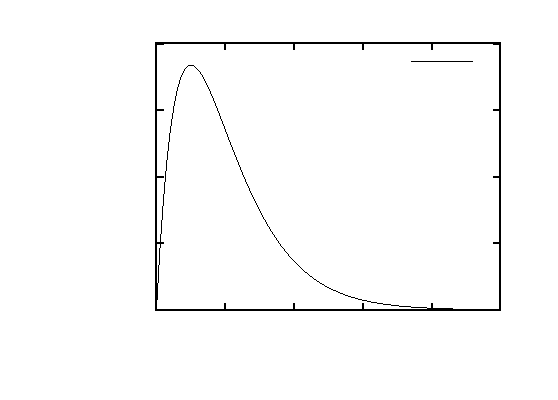
\includegraphics{alpha}}%
    \gplfronttext
  \end{picture}%
\endgroup

\end{center}
\caption{The $\alpha$-function profile often used to model synaptic
  conductances, shown here with $\tau_m=10$ ms.\label{fig:alpha}}
\end{figure}

The basic idea is that a closed ligand gated channel has a probability
of opening which depends on the concentration of the
neurotransmitter. Lets call this opening rate $o$; since the level of
neurotransmitter varies, $o(t)$. Conversely when a channel is open
there is a chance the neurotransmitter will unbind because of thermal
fluctuations, lets call this closing rate $c$, $c$ is a constant. Now
if $x$ is the fraction of gates that are open
\begin{equation}
\frac{dx}{dt}=(1-x)o-xc
\end{equation}
since $(1-x)$ is the number of open gates and $o$ is the opening rate.

Now we need to have some description of how $o$ varies with time. One
idea is that $o$ might be an exponential: perhaps the more
neurotransmitter there is the faster it gets transported away by the
neurotransmitter reuptake pumps. Let
\begin{equation}
o(t)=\bar{o}e^{-t/\tau_o}
\end{equation}
in response to a spike at time $t=0$. Hence
\begin{equation}
\frac{dx}{dt}+(\bar{o}e^{-t/\tau_o}+c)x=\bar{o}e^{-t/\tau_o}
\end{equation}
Clearly this is going to be a complete pain to solve, we can make it easier with a few approximations, say $c>>\bar{o}$, that is, because of the decay in the exponential, the coefficient of $x$ is quickly dominated by $c$
\begin{equation}
\frac{dx}{dt}+cx=\bar{o}e^{-t/\tau_o}
\end{equation}
This can be solved, it is an inhomogenous first order differential
equation and using an integrating factor the solution with $x(0)=0$ is
\begin{equation}
x(t)=\tau_o\bar{o}\left(e^{-ct}-e^{-t/tau_o}\right)
\end{equation}

This is quite complicated, it has three timescales in it, $\tau_o$,
the decay time for the neurotransmitter, the maximum opening rate
$1/\bar{o}$ and the closing rate $1/c$. Often this is simplified by
assuming $1/c=\tau_o$, there is no particular reason for doing this
except that, maybe, the precise shape, as opposed to amplitude or
overall duration, of the synapse conductance does not have much
consequence and so it is reasonable to simplify. If $1/c=\tau_o$ the
equation becomes
\begin{equation}
\frac{dx}{dt}+cx=\bar{o}e^{-ct}
\end{equation}
and the previous solution is uniformly zero. In the language of
ordinary differential equations this is called the critically damped
case. It can also be solved by integating factor, multiplying both
sides by $\exp{(ct)}$ gives
\begin{equation}
e^{ct}\frac{dx}{dt}+ce^{ct}x=\bar{o}
\end{equation}
or
\begin{equation}
\frac{d}{dt}\left[e^{ct}x\right]=\bar{o}
\end{equation}
Integrating gives
\begin{equation}
x(t)=\bar{o}te^{-ct}+Ae^{-ct}
\end{equation}
where $A$ is an integration constant that gets set to zero if
$x(0)=0$. Thus, there is a derivation for the $\alpha$ function, just not a paritcularly good one!

Another model describes the period of time that the neurotransmitter
is in the cleft as a square pulse, this might not be all that
realistic either, but it is a simplification that makes it easier to
deal with how the conductance changes in response to more than one
spike. Say there is a spike at $t=0$:
\begin{equation}
o(t)=\left\{\begin{array}{ll}\bar{o}&0<t<\tau_o\\0&\mbox{otherwise}\end{array}\right.
\end{equation}
Imagine $\bar{o}$ is much bigger than $c$ so that in $0<t<\tau_o$ 
\begin{equation}
\frac{dx}{dt}=(1-x)\bar{o}=-\bar{o}x-\bar{o}
\end{equation}
We can solve this:
\begin{equation}
x(t)=\bar{o}+[x(0)-\bar{o}]e^{-\bar{o}t}
\end{equation}
For $t>\tau_o$ 
\begin{equation}
\frac{dx}{dt}=-cx
\end{equation}
so 
\begin{equation}
x(t)=x(\tau_o)e^{-ct}
\end{equation}

Now, a useful approximation here is to ignore the short time $o$ is
non-zero, in other words, to assume that the dynamics during the
period the cleft is full of neurotransmitter is uninteresting, we have
in any case approximated it rather crudely. Now between the spike
arriving and the end of this short period $x(t)$ has gone from $x(0)$ to
\begin{equation}
x(\tau_o)=\bar{o}+[x(0)-\bar{o}]e^{-\bar{o}t}
\end{equation}
which can be rearranged to give
\begin{equation}
x(\tau_o)=x(0)+[\bar{o}-x(0)]\left(1-e^{-\bar{o}t}\right)
\end{equation}
If there hasn't be a spike in a long time $x(0)=0$ and in that case
\begin{equation}
x(\tau_o)=\bar{o}\left(1-e^{-\bar{o}t}\right)
\end{equation}
This is actually the largest increase in the conductance that is
possible, call this value $x_m$ and substitute back into the general
equation for $x(\tau_o)$:
\begin{equation}
x(\tau_o)=x(0)+\frac{[\bar{o}-x(0)]x_m}{\bar{o}}
\end{equation}
This gives another popular model for synapses where 
\begin{equation}
\frac{dx}{dt}=-cx
\end{equation}
but every time there is a spike
\begin{equation}
x(t)\rightarrow x(t)+\frac{[\bar{o}-x(t)]x_m}{\bar{o}}
\end{equation}
This becomes a bit easier to interpret if we write $x(t)=\bar{o}p(t)$ and $x_m=\bar{o}p(t)$, then
\begin{equation}
\frac{dp}{dt}=-cp
\end{equation}
but every time there is a spike
\begin{equation}
p(t)\rightarrow p(t)+[1-p(t)]p_m
\end{equation}
and we can see that $p_m$ is the fraction of available gates that open
with each spike.


\end{document}
